\label{s:exp_realmamm_spicule_classification}
%
Although it was not realistic to create a training set of mammogram images with all spicules annotated, we were able to obtain expert annotations of a reasonably large number of spicules in a set of mammogram patches containing malignant tumours. These annotations were used to select pixels for the positive training set. 

To create a balanced training set we sampled feature vectors from the same number of pixels in a set of normal mammogram patches, such that the distribution of curvilinear structure probabilities was the same as for the spicule training set.

Having trained a classifier using the synthetic data, we can classify feature vectors extracted about every pixel in a synthetic or real mammogram image to obtain a line probability image (using the probabilistic labelling scheme as opposed to a hard binary classification).

The four learning-based methods were also applied to the problem of spicule/non-spicule classification. Feature vectors were formed as above, and random forest classifiers were trained using balanced spicule/non-spicule training data. 

% Cross validation
To make effective use of the available data, we used a 10-fold cross validation design. The set of normal and abnormal regions were divided into 10 groups so that the total number of normal and spicule pixels in each group were as close as possible to one tenth of the total and no two views from the same case were included in different groups. The samples in each group were then classified using a random forest trained on the samples from the remaining 9 groups. The classification results from each group were pooled to generate an unbiased class probability for each sampled pixel. 

These probabilities were used to compute an ROC curve for each training regime, and the area under the curve ($A_z$) was computed and used as a measure of classification performance. The ROC curves and $A_z$ values for the three methods are shown in \ref{f:} and \ref{t:}. These results demonstrate a clear advantage for \dtcwt{}/RF. Linop and Gaussian representations perform significantly worse than the two representations that do include phase; we believe that this is because phase information captures profile shape.

In addition to computing a class vote for spicule membership at only those pixels in the selected training sets, the forests we have constructed can be used to compute results for whole region in each cross-fold group. Typical qualitative \dtcwt{}/RF results for a normal and abnormal region are shown in \ref{f:}. In the left column, the original regions are shown. The spiculations of the mass are clear and well defined, particularly to the lower right of the central mass. In the normal region, a set of structures intersect in an approximate radial pattern that may trigger a feature detector erroneously. In the right column, the predicted spicule class membership is shown as hue varying from cyan (normal) to pink (spicule), modulated by the \textbf{output of the \dtcwt{}/RF detection method}. Note how the linear structures in the region of the mass are deemed highly likely to be spicules, while those in the normal region are not. 
%This shows excellent promise as a means of providing a relevance measure to methods for abnormality detection.

% IMPI Figure 5

\begin{figure}
\centering
\begin{tabular}{c c}
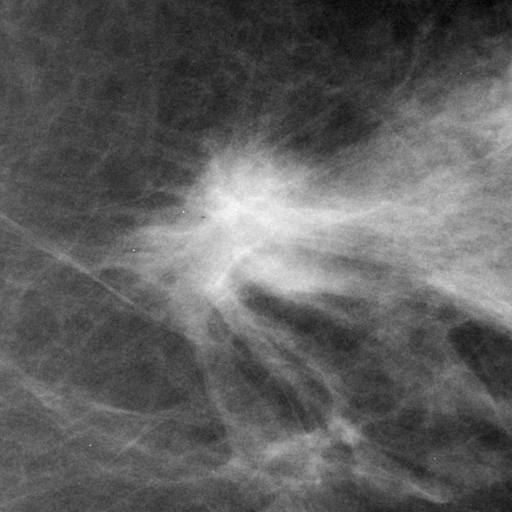
\includegraphics[width=\qtrcol]{\figpath/mammo/ipmi/mass046} &
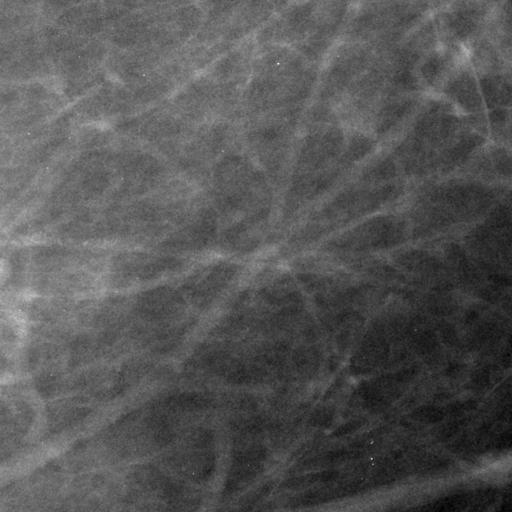
\includegraphics[width=\qtrcol]{\figpath/mammo/ipmi/norm068} \\
(a) & (b) \\
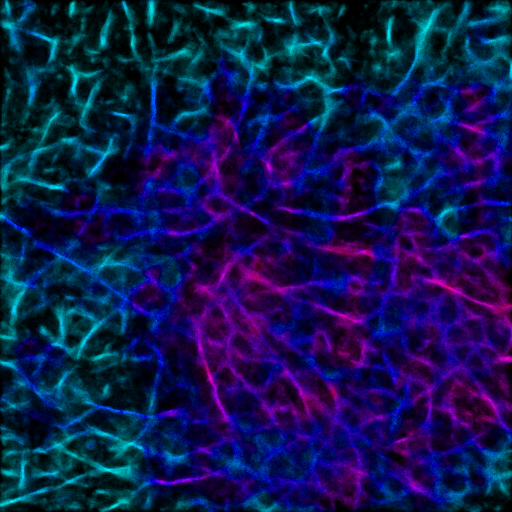
\includegraphics[width=\qtrcol]{\figpath/mammo/ipmi/spic_prob_mass046_a} &
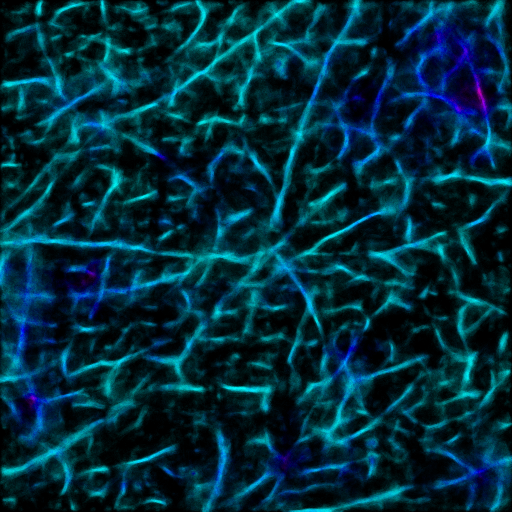
\includegraphics[width=\qtrcol]{\figpath/mammo/ipmi/spic_prob_norm068_a} \\
(c) & (d)
\end{tabular}
%
\caption{Regions depicting (a) malignant and (b) normal tissue. The corresponding spicule classification results are depicted in (c,d) using hue to indicate abnormality -- ranging from cyan (normal) to pink (spicule) -- and intensity to indicate the line detection output from the DT-CWT method.}
\label{f:mammogram_examples}
\end{figure}

